% pipeline_phase2.tex — Phase 2: intonation and vibrato (not yet implemented).
% Standalone TikZ; compile with:  pdflatex pipeline_phase2.tex
\documentclass[tikz,border=6pt]{standalone}
\usepackage{amsmath,amssymb}
\usetikzlibrary{positioning,arrows.meta,fit,backgrounds}

\definecolor{ink}{HTML}{1A1A1A}
\definecolor{muted}{HTML}{6B7280}
\definecolor{rule}{HTML}{9CA3AF}
\definecolor{accent}{HTML}{9A3324}

\begin{document}
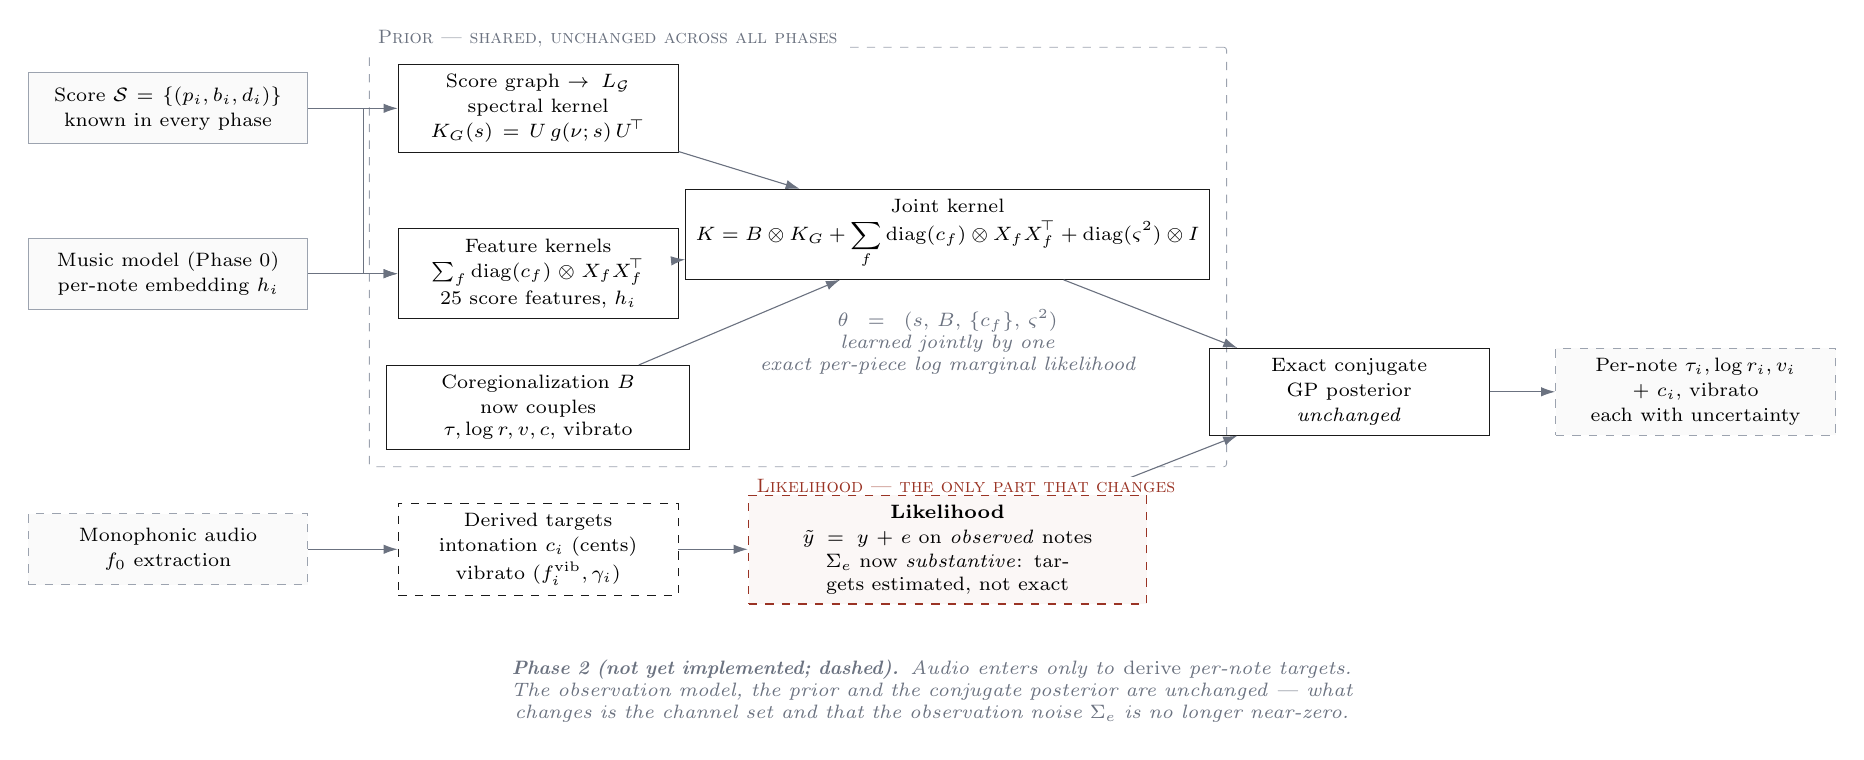
\begin{tikzpicture}[
  font=\scriptsize,
  box/.style   = {draw=ink, line width=0.35pt, align=center, inner sep=3.6pt,
                  text width=33mm, minimum height=9mm},
  io/.style    = {box, draw=rule, fill=black!2},
  new/.style   = {box, draw=ink, dashed, line width=0.35pt},
  newio/.style = {io, dashed},
  acc/.style   = {box, draw=accent, dashed, line width=0.6pt, fill=accent!4},
  arr/.style   = {-{Latex[length=1.8mm,width=1.2mm]}, draw=muted, line width=0.4pt},
  note/.style  = {font=\scriptsize\itshape, text=muted, align=center},
  grouplab/.style = {font=\scriptsize\scshape, text=muted, fill=white, inner xsep=3pt, inner ysep=1pt},
]

% ---------- inputs ----------
\node[io] (score) at (0,2.5)
  {Score $\mathcal{S}=\{(p_i,b_i,d_i)\}$\\[1pt] known in every phase};
\node[io] (mm) at (0,0.4)
  {Music model (Phase 0)\\[1pt] per-note embedding $h_i$};
\node[newio] (obs) at (0,-3.1)
  {Monophonic audio\\[1pt] $f_0$ extraction};

% ---------- prior construction (unchanged) ----------
\node[box] (gk) at (4.7,2.5)
  {Score graph $\to L_{\mathcal G}$\\[1pt] spectral kernel\\[1pt] $K_G(s)=U\,g(\nu;s)\,U^{\!\top}$};
\node[box] (fk) at (4.7,0.4)
  {Feature kernels\\[1pt] $\textstyle\sum_f \operatorname{diag}(c_f)\otimes X_fX_f^{\!\top}$\\[1pt] 25 score features, $h_i$};
\node[box, text width=36mm] (cor) at (4.7,-1.3)
  {Coregionalization $B$\\[1pt] now couples $\tau,\log r,v,c$, vibrato};

\node[box, text width=64mm] (K) at (9.9,0.9)
  {Joint kernel\\[2pt]
   $K=B\otimes K_G+\displaystyle\sum_f \operatorname{diag}(c_f)\otimes X_fX_f^{\!\top}+\operatorname{diag}(\varsigma^2)\otimes I$};

% ---------- new channels + likelihood ----------
\node[new] (tgt) at (4.7,-3.1)
  {Derived targets\\[1pt] intonation $c_i$ (cents)\\[1pt] vibrato $(f_i^{\mathrm{vib}},\gamma_i)$};
\node[acc, text width=48mm] (lik) at (9.9,-3.1)
  {\textbf{Likelihood}\\[1pt] $\tilde y = y + e$ on \emph{observed} notes\\[1pt]
   $\Sigma_e$ now \emph{substantive}: targets estimated, not exact};

% ---------- inference + outputs ----------
\node[box] (inf) at (15.0,-1.1)
  {Exact conjugate\\[1pt] GP posterior\\[1pt] \emph{unchanged}};
\node[newio] (out) at (19.4,-1.1)
  {Per-note $\tau_i,\log r_i,v_i$\\[1pt] $+\ c_i$, vibrato\\[1pt] each with uncertainty};

% ---------- arrows ----------
\draw[arr] (score) -- (gk);
\draw[arr] (score.east) -- ++(0.7,0) |- (fk.west);
\draw[arr] (mm) -- (fk);
\draw[arr] (gk) -- (K);
\draw[arr] (fk) -- (K);
\draw[arr] (cor) -- (K);
\draw[arr] (obs) -- (tgt);
\draw[arr] (tgt) -- (lik);
\draw[arr] (K) -- (inf);
\draw[arr] (lik) -- (inf);
\draw[arr] (inf) -- (out);

% ---------- annotations ----------
\node[note, below=2.5mm of K, text width=52mm]
  {$\theta=(s,\,B,\,\{c_f\},\,\varsigma^2)$ learned jointly by one\\ exact per-piece log marginal likelihood};

\begin{scope}[on background layer]
  \node[draw=rule, dashed, line width=0.3pt, rounded corners=1pt,
        fit=(gk)(fk)(cor)(K), inner sep=6pt] (prior) {};
\end{scope}
\node[grouplab, above=1mm of prior.north west, anchor=west]
  {Prior --- shared, unchanged across all phases};
\node[grouplab, text=accent, above=1mm of lik.north west, anchor=west]
  {Likelihood --- the only part that changes};

\node[note, text width=150mm] at (9.7,-4.9)
  {\textbf{Phase 2 (not yet implemented; dashed).} Audio enters only to \emph{derive} per-note targets.
   The observation model, the prior and the conjugate posterior are unchanged --- what changes is the
   channel set and that the observation noise $\Sigma_e$ is no longer near-zero.};

\end{tikzpicture}
\end{document}
